
\documentclass[letterpaper,hide notes,xcolor={table,svgnames},pdftex,10pt]{beamer}
\def\showexamples{t}

\usecolortheme{crane}
\setbeamertemplate{navigation symbols}{}

\usetheme{MyPittsburgh}
\usepackage{hyperref}
\usepackage{graphicx,xspace}
\usepackage[normalem]{ulem}
\usepackage{multicol}
\usepackage{amsmath,amssymb,amsthm,graphicx,xspace}
\newcommand\SF[1]{$\bigstar$\footnote{SF: #1}}

\usepackage[sfdefault,lf]{carlito}
\usepackage[T1]{fontenc}
\usepackage[scaled]{beramono}
\usepackage{tikzpagenodes}
\newcommand{\Rplus}{\protect\hspace{-.1em}\protect\raisebox{.35ex}{\small{\small\textbf{+}}}}
\newcommand{\Cpp}{\mbox{C\Rplus\Rplus}\xspace}

\newcounter{tmpnumSlide}
\newcounter{tmpnumNote}

\newcommand\mnote[1]{%
	\addtocounter{tmpnumSlide}{1}
	\ifdefined\showcues {~\tiny\fbox{\arabic{tmpnumSlide}}}\fi
	\note{\setlength{\parskip}{1ex}\addtocounter{tmpnumNote}{1}\textbf{\Large \arabic{tmpnumNote}:} {#1\par}}}

\newcommand\mmnote[1]{\note{\setlength{\parskip}{1ex}#1\par}}


\newcommand\mquestion[2]{{~\color{red}\fbox{?}}\note{\setlength{\parskip}{1ex}\par{\Large \textbf{?}} #1} \note{\setlength{\parskip}{1ex}\par{\Large \textbf{A}} #2\par}\ifdefined \presentationonly \pause \fi}

\newcommand\blackboard[1]{%
	\ifdefined   \showblackboard
		{#1}
	\else {\begin{center} \fbox{\colorbox{blue!30}{%
						\begin{minipage}{.95\linewidth}%
							\hspace{\stretch{1}} Some space intentionally left blank; done at the blackboard.%
						\end{minipage}}}\end{center}}%
	\fi%
}

\usepackage{listings}
\lstset{%
	keywordstyle=\bfseries,
	aboveskip=15pt,
	belowskip=15pt,
	captionpos=b,
	identifierstyle=\ttfamily,
	frame=lines,
	numbers=left, basicstyle=\scriptsize, numberstyle=\tiny, stepnumber=0, numbersep=2pt}

\usepackage{siunitx}
\newcommand\sius[1]{\num[group-separator = {,}]{#1}\si{\micro\second}}
\newcommand\sims[1]{\num[group-separator = {,}]{#1}\si{\milli\second}}
\newcommand\sins[1]{\num[group-separator = {,}]{#1}\si{\nano\second}}
\sisetup{group-separator = {,}, group-digits = true}

%% -------------------- tikz --------------------
\usepackage{tikz}
\usetikzlibrary{positioning}
\usetikzlibrary{arrows,backgrounds,automata,decorations.shapes,decorations.pathmorphing,decorations.markings,decorations.text}

\tikzstyle{place}=[circle,draw=blue!50,fill=blue!20,thick, inner sep=0pt,minimum size=6mm]
\tikzstyle{transition}=[rectangle,draw=black!50,fill=black!20,thick, inner sep=0pt,minimum size=4mm]

\tikzstyle{block}=[rectangle,draw=black, thick, inner sep=5pt]
\tikzstyle{bullet}=[circle,draw=black, fill=black, thin, inner sep=2pt]

\tikzstyle{pre}=[<-,shorten <=1pt,>=stealth',semithick]
\tikzstyle{post}=[->,shorten >=1pt,>=stealth',semithick]
\tikzstyle{bi}=[<->,shorten >=1pt,shorten <=1pt, >=stealth',semithick]

\tikzstyle{mut}=[-,>=stealth',semithick]

\tikzstyle{treereset}=[dashed,->, shorten >=1pt,>=stealth',thin]

\usepackage{ifmtarg}
\usepackage{xifthen}
\makeatletter
% new counter to now which frame it is within the sequence
\newcounter{multiframecounter}
% initialize buffer for previously used frame title
\gdef\lastframetitle{\textit{undefined}}
% new environment for a multi-frame
\newenvironment{multiframe}[1][]{%
	\ifthenelse{\isempty{#1}}{%
		% if no frame title was set via optional parameter,
		% only increase sequence counter by 1
		\addtocounter{multiframecounter}{1}%
	}{%
		% new frame title has been provided, thus
		% reset sequence counter to 1 and buffer frame title for later use
		\setcounter{multiframecounter}{1}%
		\gdef\lastframetitle{#1}%
	}%
	% start conventional frame environment and
	% automatically set frame title followed by sequence counter
	\begin{frame}%
		\frametitle{\lastframetitle~{\normalfont(\arabic{multiframecounter})}}%
		}{%
	\end{frame}%
}
\makeatother

\makeatletter
\newdimen\tu@tmpa%
\newdimen\ydiffl%
\newdimen\xdiffl%
\newcommand\ydiff[2]{%
	\coordinate (tmpnamea) at (#1);%
	\coordinate (tmpnameb) at (#2);%
	\pgfextracty{\tu@tmpa}{\pgfpointanchor{tmpnamea}{center}}%
	\pgfextracty{\ydiffl}{\pgfpointanchor{tmpnameb}{center}}%
	\advance\ydiffl by -\tu@tmpa%
}
\newcommand\xdiff[2]{%
	\coordinate (tmpnamea) at (#1);%
	\coordinate (tmpnameb) at (#2);%
	\pgfextractx{\tu@tmpa}{\pgfpointanchor{tmpnamea}{center}}%
	\pgfextractx{\xdiffl}{\pgfpointanchor{tmpnameb}{center}}%
	\advance\xdiffl by -\tu@tmpa%
}
\makeatother
\newcommand{\copyrightbox}[3][r]{%
	\begin{tikzpicture}%
		\node[inner sep=0pt,minimum size=2em](ciimage){#2};
		\usefont{OT1}{phv}{n}{n}\fontsize{4}{4}\selectfont
		\ydiff{ciimage.south}{ciimage.north}
		\xdiff{ciimage.west}{ciimage.east}
		\ifthenelse{\equal{#1}{r}}{%
			\node[inner sep=0pt,right=1ex of ciimage.south east,anchor=north west,rotate=90]%
			{\raggedleft\color{black!50}\parbox{\the\ydiffl}{\raggedright{}#3}};%
		}{%
			\ifthenelse{\equal{#1}{l}}{%
				\node[inner sep=0pt,right=1ex of ciimage.south west,anchor=south west,rotate=90]%
				{\raggedleft\color{black!50}\parbox{\the\ydiffl}{\raggedright{}#3}};%
			}{%
				\node[inner sep=0pt,below=1ex of ciimage.south west,anchor=north west]%
				{\raggedleft\color{black!50}\parbox{\the\xdiffl}{\raggedright{}#3}};%
			}
		}
	\end{tikzpicture}
}


%% --------------------

%\usepackage[excludeor]{everyhook}
%\PushPreHook{par}{\setbox0=\lastbox\llap{MUH}}\box0}

%\vspace*{\stretch{1}

%\setbox0=\lastbox \llap{\textbullet\enskip}\box0}

\setlength{\parskip}{\fill}

\newcommand\noskips{\setlength{\parskip}{1ex}}
\newcommand\doskips{\setlength{\parskip}{\fill}}

\newcommand\xx{\par\vspace*{\stretch{1}}\par}
\newcommand\xxs{\par\vspace*{2ex}\par}
\newcommand\tuple[1]{\langle #1 \rangle}
\newcommand\code[1]{{\sf \footnotesize #1}}
\newcommand\ex[1]{\uline{Example:} \ifdefined \presentationonly \pause \fi
	\ifdefined\showexamples#1\xspace\else{\uline{\hspace*{2cm}}}\fi}

\newcommand\ceil[1]{\lceil #1 \rceil}


\AtBeginSection[]
{
	\begin{frame}
		\frametitle{Outline}
		\tableofcontents[currentsection]
	\end{frame}
}



\pgfdeclarelayer{edgelayer}
\pgfdeclarelayer{nodelayer}
\pgfsetlayers{edgelayer,nodelayer,main}

\tikzstyle{none}=[inner sep=0pt]
\tikzstyle{rn}=[circle,fill=Red,draw=Black,line width=0.8 pt]
\tikzstyle{gn}=[circle,fill=Lime,draw=Black,line width=0.8 pt]
\tikzstyle{yn}=[circle,fill=Yellow,draw=Black,line width=0.8 pt]
\tikzstyle{empty}=[circle,fill=White,draw=Black]
\tikzstyle{bw} = [rectangle, draw, fill=blue!20,
text width=4em, text centered, rounded corners, minimum height=2em]

\newcommand{\CcNote}[1]{% longname
	This work is licensed under the \textit{Creative Commons #1 3.0 License}.%
}
\newcommand{\CcImageBy}[1]{%
	\includegraphics[scale=#1]{creative_commons/cc_by_30.pdf}%
}
\newcommand{\CcImageSa}[1]{%
	\includegraphics[scale=#1]{creative_commons/cc_sa_30.pdf}%
}
\newcommand{\CcImageNc}[1]{%
	\includegraphics[scale=#1]{creative_commons/cc_nc_30.pdf}%
}
\newcommand{\CcGroupBySa}[2]{% zoom, gap
	\CcImageBy{#1}\hspace*{#2}\CcImageNc{#1}\hspace*{#2}\CcImageSa{#1}%
}
\newcommand{\CcLongnameByNcSa}{Attribution-NonCommercial-ShareAlike}

\newenvironment{changemargin}[1]{% 
	\begin{list}{}{% 
		\setlength{\topsep}{0pt}% 
		\setlength{\leftmargin}{#1}% 
		\setlength{\rightmargin}{1em}
		\setlength{\listparindent}{\parindent}% 
		\setlength{\itemindent}{\parindent}% 
		      \setlength{\parsep}{\parskip}% 
		      }% 
		\item[]}{\end{list}}




\title{Lecture 4 --- Processes }

\author{Jeff Zarnett \\ \small \texttt{jzarnett@uwaterloo.ca}}
\institute{Department of Electrical and Computer Engineering \\
	University of Waterloo}
\date{\today}


\begin{document}

\begin{frame}
	\titlepage

\end{frame}

\begin{frame}
	\frametitle{Processes}


	Early computers did exactly one thing.

	Or at least, exactly one thing at a time.

	Now the OS supports multiple programs running concurrently.

	To manage this complexity, the OS uses the \alert{process}.

\end{frame}

\begin{frame}
	\frametitle{The Process}

	A process is a program in execution.

	\begin{enumerate}
		\item The instructions and data.
		\item The current state.
		\item Any resources that are needed to execute.
	\end{enumerate}

\end{frame}


\begin{frame}
	\frametitle{Processes vs. Programs}

	Note: two instances of the same program running equals two processes.

	You may have two windows open for Microsoft Word, and even though they are the same program, they are separate processes.


	Similarly, two users who both use Firefox at the same time on a terminal server are interacting with two different processes.

\end{frame}


\begin{frame}
	\frametitle{Two Documents, Two Processes}

	\begin{center}
		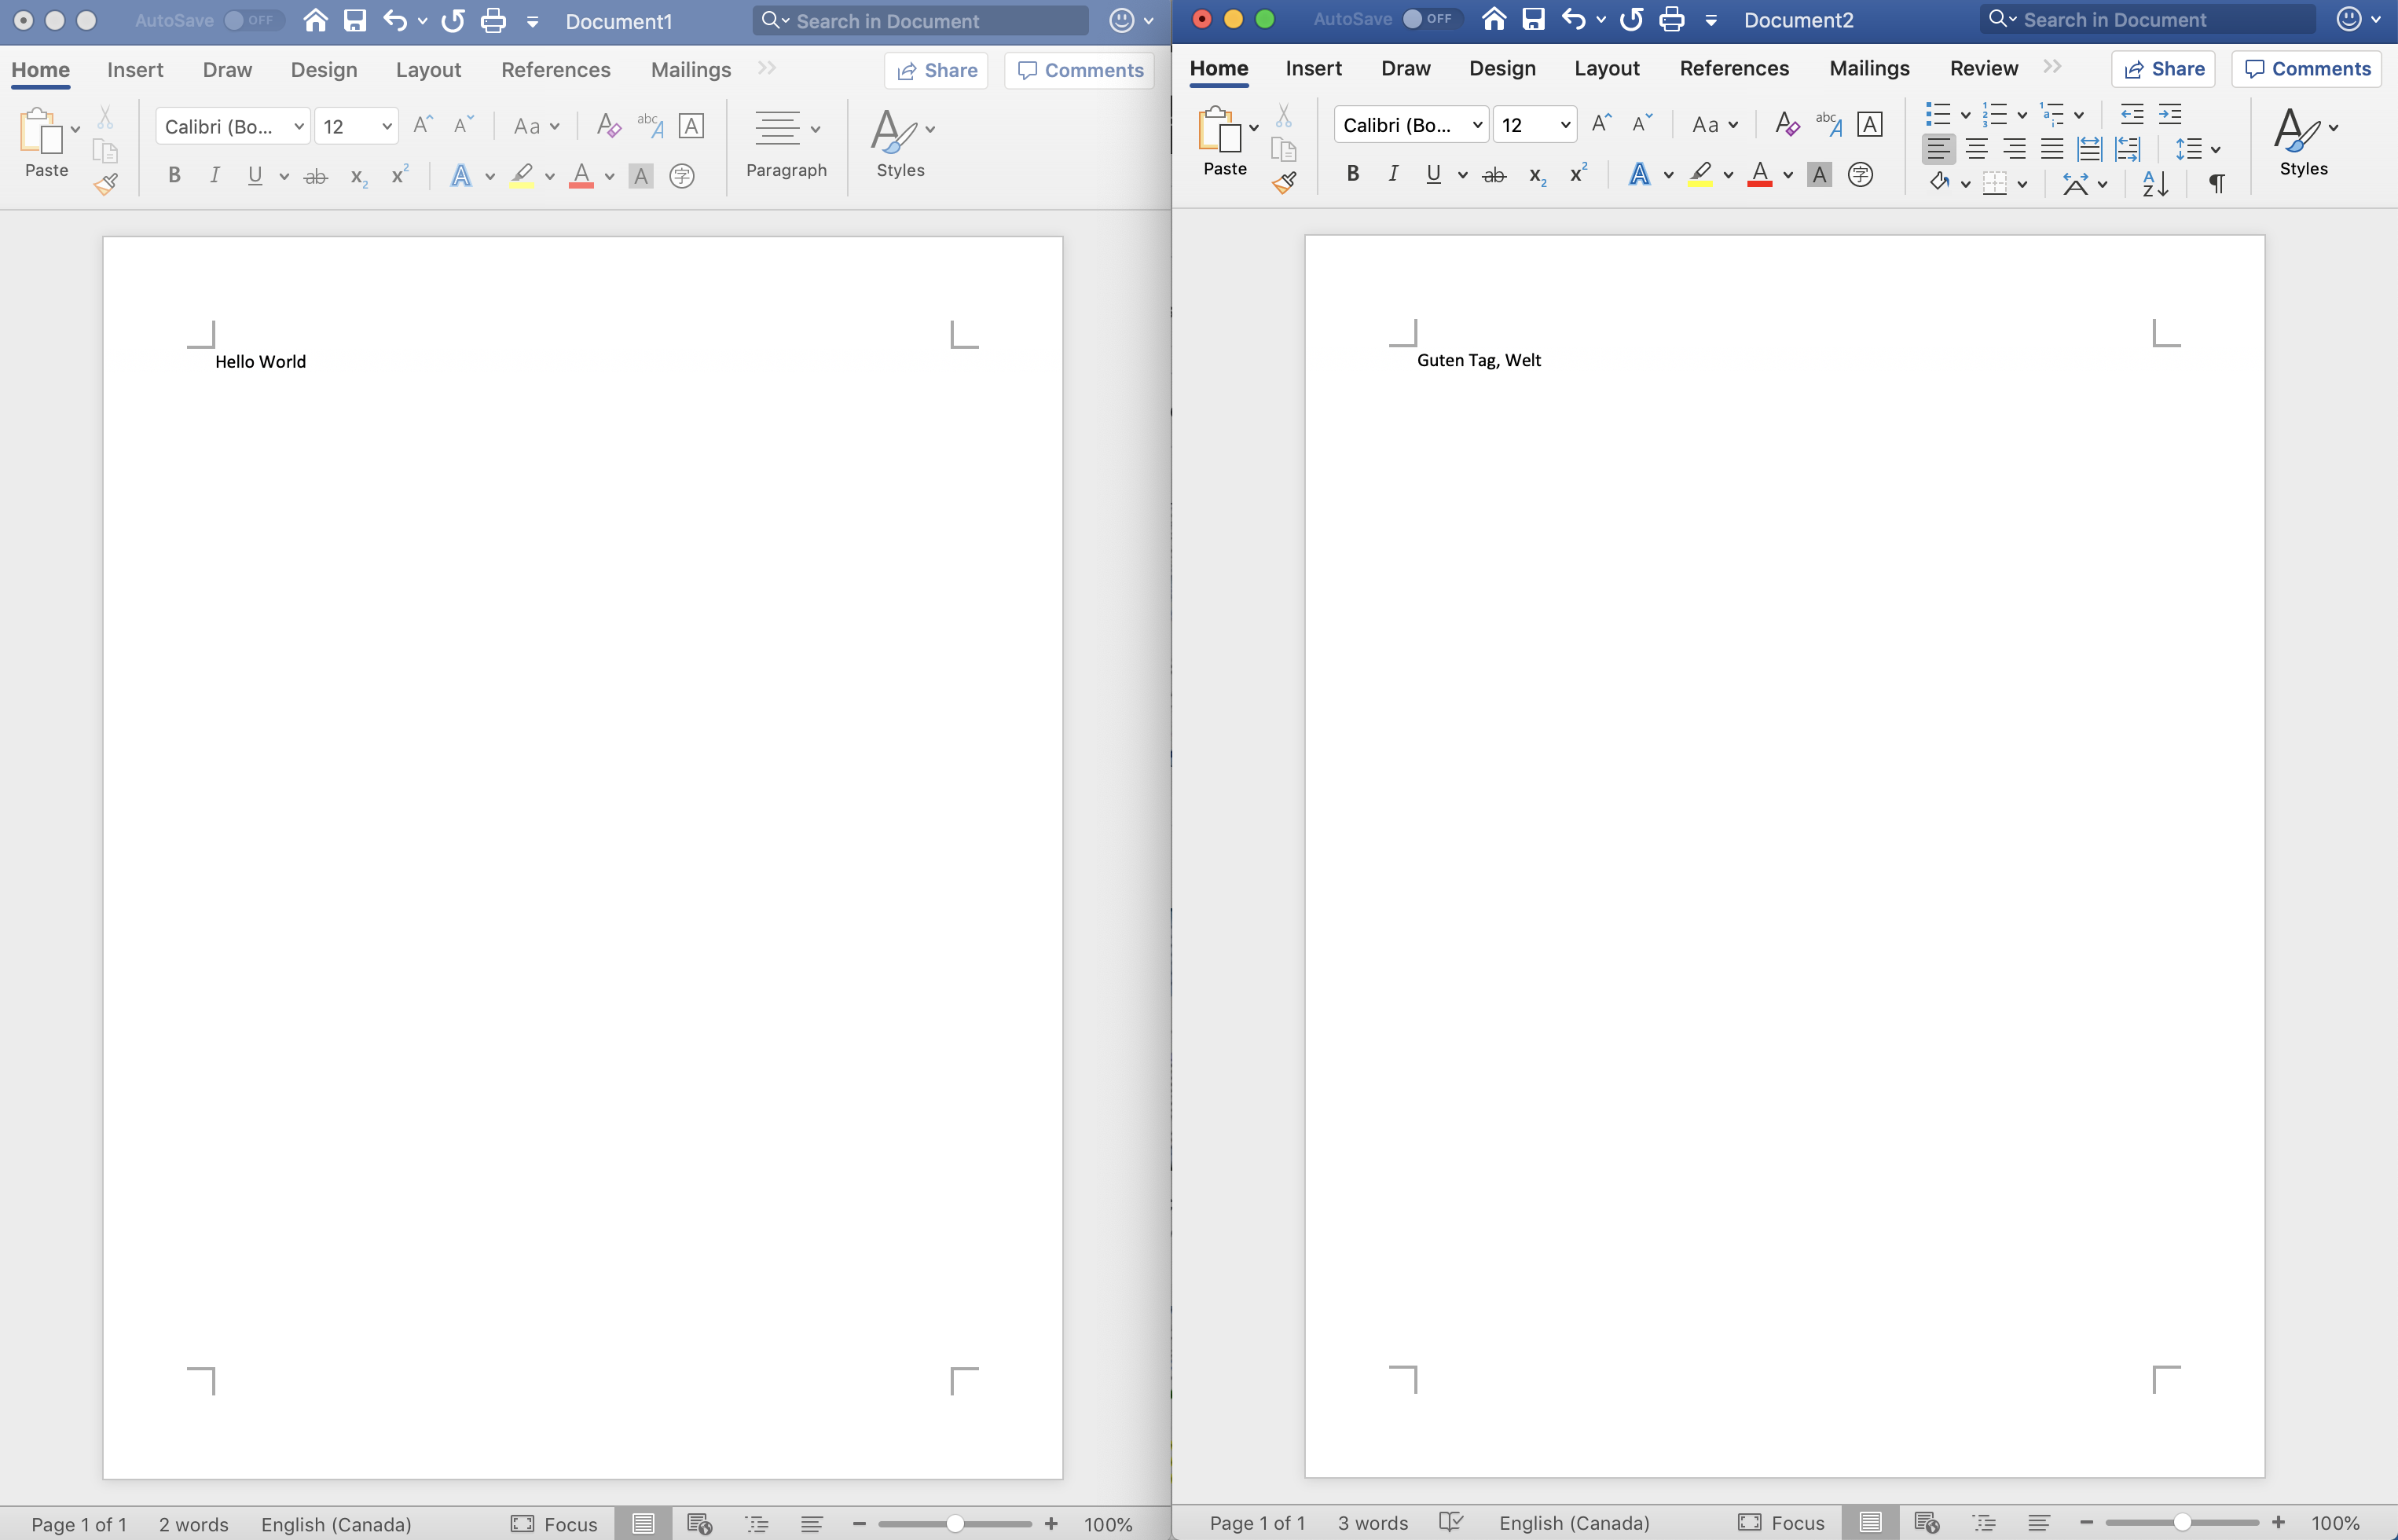
\includegraphics[width=\textwidth]{images/2docs.png}
	\end{center}


\end{frame}


\begin{frame}
	\frametitle{Process Control Block}

	Data structure for managing processes: \alert{Process Control Block} (PCB).

	It contains everything the OS needs to know about the program.

	It is created and updated by the OS for each running process.

	It can be thrown away when the program has finished executing and cleaned everything up.

	The blocks are held in memory and maintained in some container (e.g., a list) by the kernel.


\end{frame}

\begin{frame}
	\frametitle{Process Control Block}

	The process control block will (usually) have:
	\begin{itemize}
		\item \textbf{Identifier.}
		\item \textbf{State.}
		\item \textbf{Priority.}
		\item \textbf{Program Counter*.}
		\item \textbf{Register Data*.}
		\item \textbf{Memory Pointers.}
		\item \textbf{I/O Status Information.}
		\item \textbf{Accounting Information.}
	\end{itemize}

\end{frame}

\begin{frame}
	\frametitle{Process Control Block (Simplified)}

	\begin{center}
		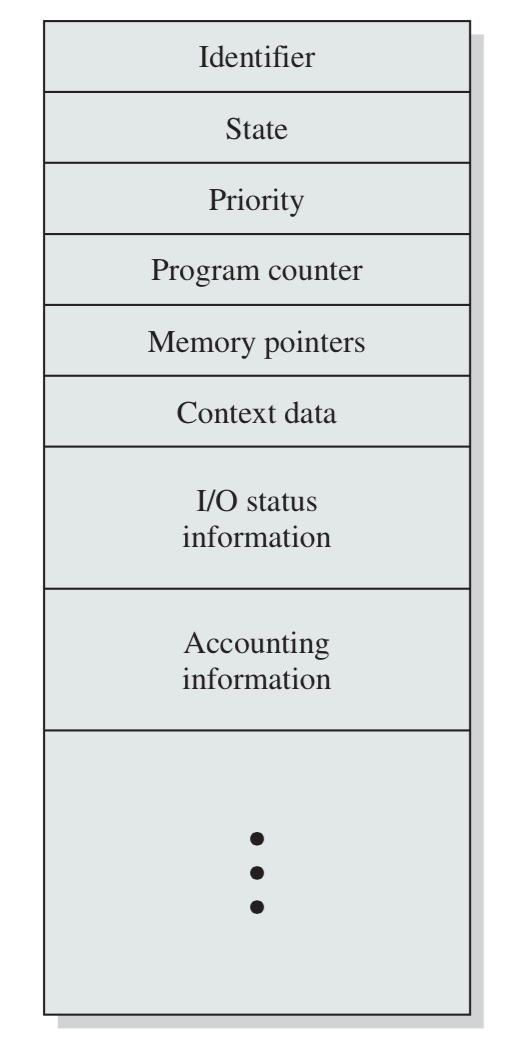
\includegraphics[width=0.35\textwidth]{images/pcb.png}
	\end{center}

\end{frame}

\begin{frame}
	\frametitle{Process Control Block}

	This data is kept up to date constantly as the process executes.

	The program counter and the register data are asterisked.

	When the program is running, these values do not need to be updated.

	They are needed when a system call (trap) or process switch occurs.

\end{frame}

\begin{frame}
	\frametitle{PCB: Asterisked Fields}
	We will need a way to restore the state of the program.

	Save the state of the process into the PCB.

	1. Save the state into the Program Counter variable.

	2. Save the Register variables.

\end{frame}

\begin{frame}
	\frametitle{Process Switch}

	A switch between the execution of process $P_{0}$ and process $P_{1}$:

	\begin{center}
		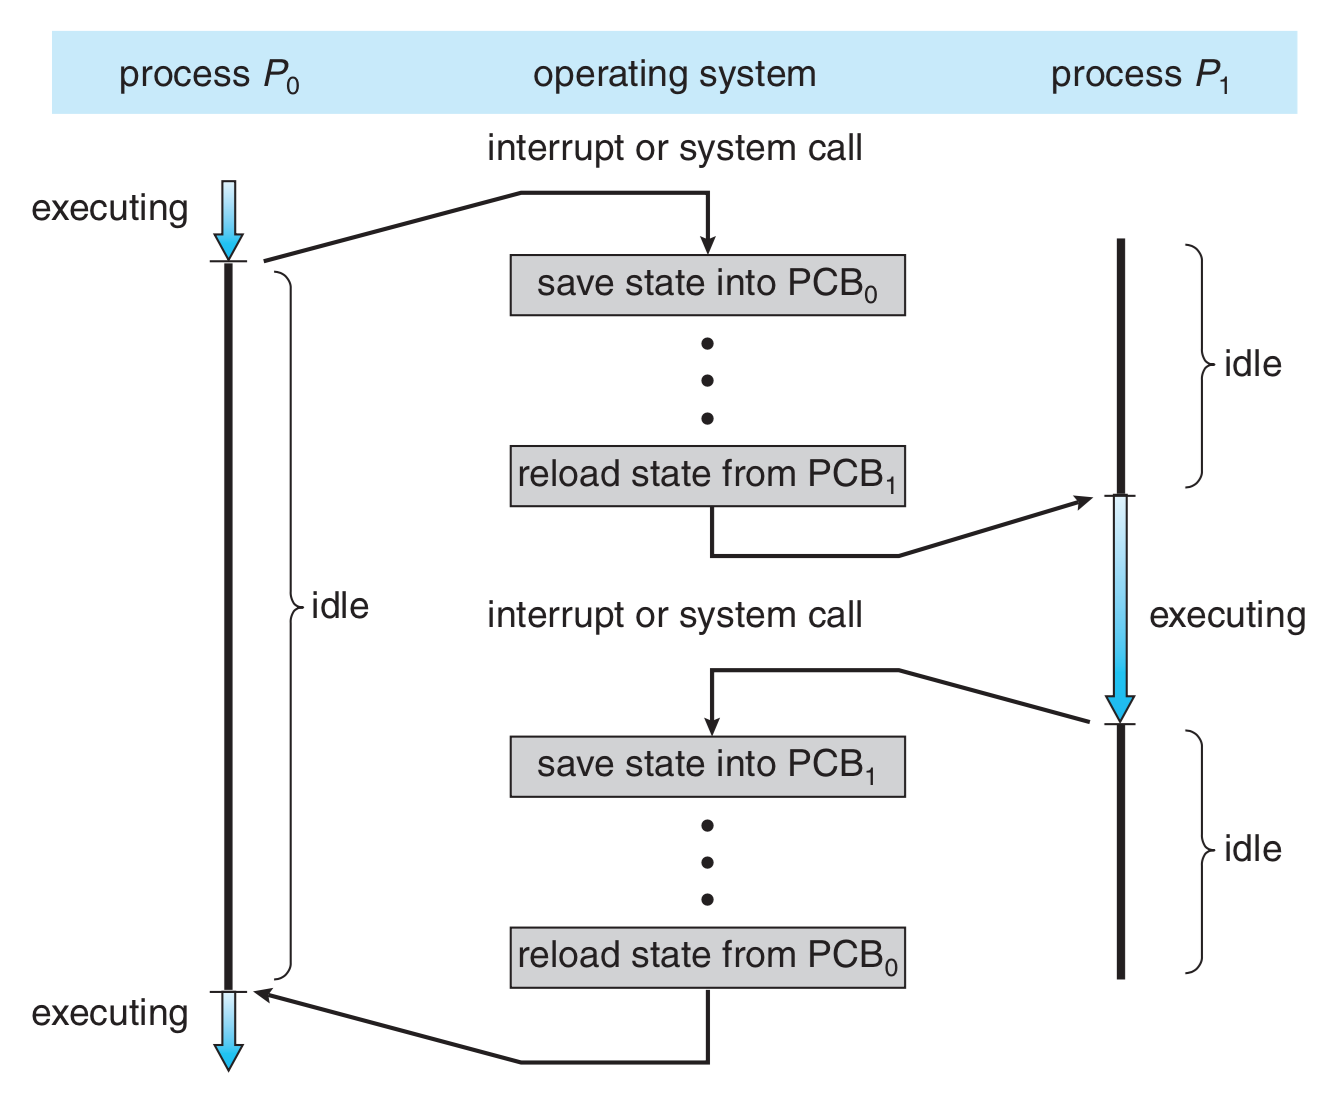
\includegraphics[width=0.75\textwidth]{images/process-switch.png}
	\end{center}

\end{frame}


\begin{frame}
	\frametitle{The Circle of Life}


	Unlike energy, processes may be created and destroyed.

	Upon creation, the OS will create a new PCB for the process.\\
	\quad Also initialize the data in that block.

	Set: variables to their initial values.\\
	\quad the initial program state.\\
	\quad the instruction pointer to the first instruction in \texttt{main}

	Add the PCB to the set.

	After the program is terminated and cleaned up:\\
	\quad Collect some data (like a summary of accounting information).\\
	\quad Remove the PCB from its list of active processes and carry on.


\end{frame}

\begin{frame}
	\frametitle{Process Creation}

	Three main events that may lead to the creation of a process:

	\begin{enumerate}
		\item System boot up.
		\item User request.
		\item One process spawns another.
	\end{enumerate}


\end{frame}

\begin{frame}
	\frametitle{Process Creation: At Boot Up}

	When the computer boots up, the OS starts and creates processes.

	An embedded system might have all the processes it will ever run.

	General-purpose operating systems: allow one (both) of the other ways.


\end{frame}

\begin{frame}
	\frametitle{Process Creation: At Boot Up}

	Some processes will be in the foreground; some in the background.

	A user-visible process: log in screen.

	Background process: server that shares media on the local network.

	UNIX term for a background process is \alert{Daemon}.

	Example: \texttt{ssh} (Secure Shell) command to log into a Linux system.


\end{frame}

\begin{frame}
	\frametitle{Process Creation: Users}

	Users are well known for starting up processes whenever they feel like it.\\
	\quad Much to the chagrin of system designers everywhere.

	Every time you double-click an icon or enter a command line command (like \texttt{ssh} above) that will result in the creation of a process.


	\begin{center}
		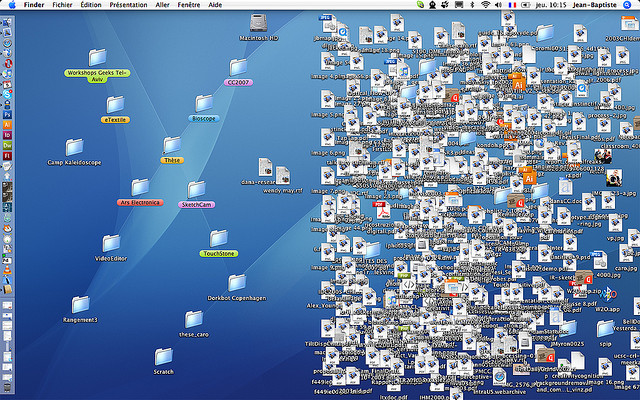
\includegraphics[width=0.6\textwidth]{images/desktop-shortcut.jpg}\\
		Image Credit: CS Tigers
	\end{center}

\end{frame}

\begin{frame}
	\frametitle{Process Creation: Spawning}

	An already-executing process may spawn another.

	E-mail with a link? Click it; the e-mail program starts the web browser.

	A program may break its work up into different logical parts.\\
	\quad To promote parallelism or fault tolerance.

	The spawning process is the \alert{parent} and the one spawned is the \alert{child}.


\end{frame}

\begin{frame}
	\frametitle{Process Destruction}

	Eventually, most processes die.

	This is sad, but it can happen in one of four ways:
	\begin{enumerate}
		\item Normal exit (voluntary)
		\item Error exit (voluntary)
		\item Fatal Error (involuntary)
		\item Killed by another process (involuntary)
	\end{enumerate}


\end{frame}

\begin{frame}
	\frametitle{Process Destruction: Normal}

	Most of the time, the process finishes because they are finished.\\
	\quad Or the user asks them to.

	Compiler: when compilation is finished, it terminates normally.

	You finish writing a document in a text editor, click the close button.

	Both examples of normal, voluntary termination.

\end{frame}

\begin{frame}
	\frametitle{Process Destruction: Error}

	Sometimes there is voluntary exit, but with an error.

	Required write access to the temporary directory \& no permission.

	Compiler: exit with an error if you ask it to compile a non-existent file.

	The program has chosen to terminate because of the error.

\end{frame}

\begin{frame}
	\frametitle{Process Destruction: Fatality}

	The third reason for termination is a fatal error.\\
	\quad Examples: stack overflow, or division by zero.

	The OS will detect this error and send it to the program.

	Often, this results in involuntary termination of the offending program.

	A process may tell the OS it wishes to handle some kinds of errors.

	If it can handle it, the process can continue.

	Otherwise, unhandled exceptions result in involuntary termination.

\end{frame}

\begin{frame}
	\frametitle{Process Destruction: Killed}

	The last reason for termination: one process might be killed by another.\\
	\quad (Yes, processes can murder one another. Is no-one safe?!).

	Typically this is a user request:\\
	\quad a program is stuck or consuming too much CPU...\\
	\quad the user opens task manager (Windows) or \texttt{ps} (UNIX)

	Programs can, without user intervention, theoretically kill other processes.

	Example: a parent process killing a child it believes to be stuck.

\end{frame}

\begin{frame}
	\frametitle{Process Destruction: Killed}

	There are restrictions on killing process.\\
	\quad A user or process must have the rights to execute the victim.

	Typically a user may only kill a process he or she has created.

	Exception: system administrator.

	While killing processes may be fun, it is something that should be reserved for when it is needed.

	Maybe when a process is killed, all processes it spawned are killed too.


\end{frame}


\begin{frame}
	\frametitle{Process Family Tree}
	In UNIX, but not in Windows, the relationship between the parent process and child process(es), if any, is maintained, forming a hierarchy.

	A process, unlike most plants and animals, reproduces asexually.

	A process has one parent; zero or more children.

	A process and all its descendants form a \alert{process group}.

	Certain operations like sending a signal can be sent to a whole group.

\end{frame}

\begin{frame}
	\frametitle{Process Family Tree: UNIX}
	UNIX the first process created is called \texttt{init}.

	It is the parent of all processes (eventually).\\
	\quad Like the \texttt{Object} class in Java is the superclass of all classes.

	Thus in UNIX we may represent all processes as a tree structure.

\end{frame}

\begin{frame}
	\frametitle{Process Family Tree: Windows}

	In Windows, a parent process gets a reference to its child.

	This allows it to exercise some measure of control over the child.

	This reference may be given to another process (adoption).

	No real hierarchy. A process in UNIX cannot disinherit a child.


\end{frame}

\begin{frame}
	\frametitle{Process Return Codes}

	When a process terminates, it does so with a return code.\\
	\quad  Just as a function often returns a value.

	On the command line or double clicking an icon, return value is ignored.

	In UNIX, a parent can get the code that process returns.

	Usually, a return value of zero indicates success.\\
	\quad Other values indicate an error of some sort.

	Normally there is some sort of understanding between the parent and child processes about what a particular code means.

\end{frame}


\begin{frame}
	\frametitle{The Walking Dead}

	\begin{center}
		
\includegraphics[width=0.8\textwidth]{images/walking-dead.jpg}
	\end{center}

\end{frame}



\begin{frame}
	\frametitle{Aaah! Zombies! Run!}

	When a child process finishes, until the parent collects the return value, the child continues in a state of ``undeath'' we call a \alert{zombie}.

	This does not mean that the process then shuffles around the system attempting to eat the brains of other processes.

	It just means that the process is dead but not gone.

	There is still an entry in the PCB list.\\
	\quad And the process holds on to its allocated resources.

	Only after the return value is collected can it be cleaned up.

\end{frame}

\begin{frame}
	\frametitle{Getting Rid of Zombies}

	Usually, a child process's result is eagerly awaited by its parent.

	The \texttt{wait} call collects the value right away.

	This allows the child to be cleaned up (or, more grimly, ``reaped'').

	If there is some delay for some reason, the process is considered a zombie until that value is collected.

\end{frame}


\begin{frame}
	\frametitle{Orphans}

	If a parent dies before the child does, the child is called an \alert{orphan}.

	In UNIX any orphan is automatically adopted by the \texttt{init} process.\\
	\quad ...making sure all processes have a good home.

	By default, \texttt{init} will just \texttt{wait} on all its child processes\\
	\quad And do nothing with the return values.

	A program can be intentionally orphaned: to run in the background.


	This would be cruel, except that processes, as far as anyone knows, do not have feelings.


\end{frame}


\begin{frame}
	\frametitle{Five State Model}

	As you might imagine, at any given time, a process is running or not running.

	The first two states of the model are therefore ``Running'' and ``Ready''.

	A program that requests a resource like I/O or memory may not get it right away.\\
	\quad This gives us the ``Blocked'' state.

\end{frame}


\begin{frame}
	\frametitle{Five State Model}

	But we did not cover things like zombies.\\
	\quad Life pro tip: the character who doubts that zombies are real dies first.

	A UNIX process may be finished but its value yet uncollected.

	It is not ready to run, but not waiting for a resource either.

\end{frame}


\begin{frame}
	\frametitle{Come with me if you want to live}

	\begin{center}
		
\includegraphics[width=0.4\textwidth]{images/judgement-day.jpg}
	\end{center}

	New state: Terminated.

\end{frame}


\begin{frame}
	\frametitle{Five State Model}
	That accounts for four states; what about the fifth?

	The fifth is the ``New'' state: just created.

	If the user creates a process, the OS has significant work to do.\\
	\quad Define an identifier.\\
	\quad Instantiate the PCB.\\
	\quad Put the process in the New state.

	The process is defined, but the OS has not started it yet.

\end{frame}

\begin{frame}
	\frametitle{Five State Model}
	Why bother with the ``New'' state?

	The system may limit the number of concurrent processes.

	New processes are typically on disk and not in memory.

\end{frame}

\begin{frame}
	\frametitle{Five State Model}

	Thus, with the two new states added, the five states are:

	\begin{enumerate}
		\item \textbf{Running}
		\item \textbf{Ready}
		\item \textbf{Blocked}
		\item \textbf{New}
		\item \textbf{Terminated}
	\end{enumerate}

\end{frame}

\begin{frame}
	\frametitle{Five State Model}

	\begin{center}
		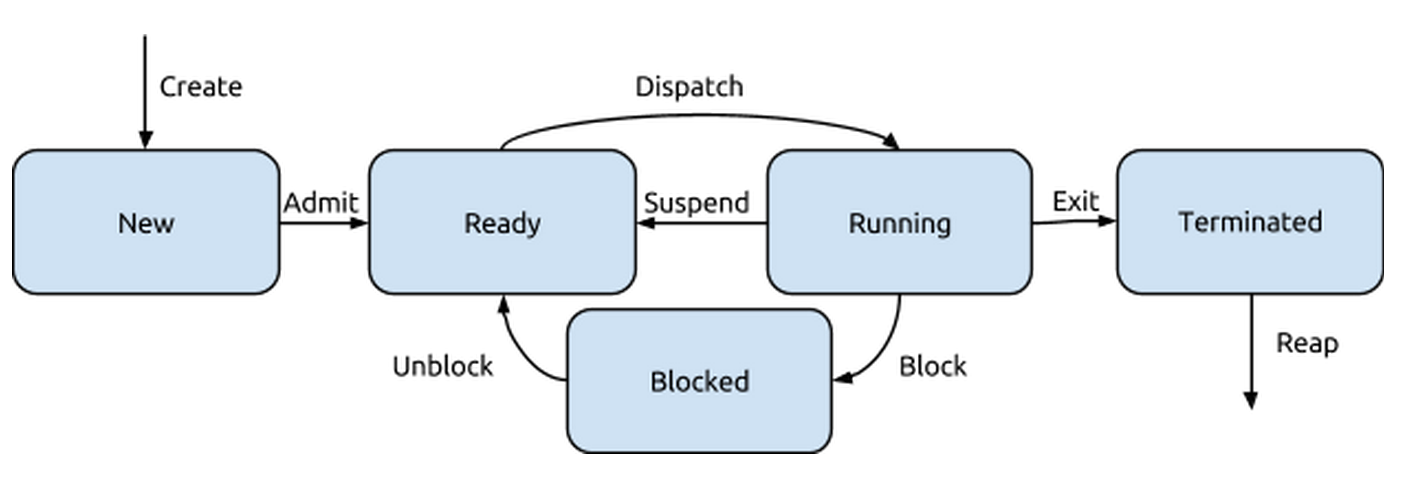
\includegraphics[width=0.9\textwidth]{images/5-state-model.png}
	\end{center}

\end{frame}

\begin{frame}
	\frametitle{Five State Model}

	There are now eight transitions:

	\begin{itemize}
		\item \textbf{Create}
		\item \textbf{Admit}
		\item \textbf{Dispatch}
		\item \textbf{Suspend}
		\item \textbf{Exit}
		\item \textbf{Block}
		\item \textbf{Unblock}
		\item \textbf{Reap}
	\end{itemize}

\end{frame}

\begin{frame}
	\frametitle{Five State Model}

	There are two additional exit transitions that are not shown.

	A process can go directly from ``Ready'' or ``Blocked'' to ``Terminated''.

	This happens if a process is killed.

\end{frame}

\begin{frame}
	\frametitle{More is the New More}

	We can expand on the five state model by considering disk.

	A process maybe swapped out to disk rather than in main memory.

	If an executing process gets blocked, maybe swap it to disk.

	Users often want more processes running than fit in memory.

	The problem is not the PCBs, but stack \& heap space of the programs.

\end{frame}

\begin{frame}
	\frametitle{The Last Resort: Disk}

	With no other place to put them, we have to put some processes on disk.

	This is what we know as \alert{swapping}.

	When the demands for memory exceed the available memory, some of the processes will be moved to disk storage to make room.

	This is a notably expensive operation.
\end{frame}

\begin{frame}
	\frametitle{Swapping to Disk}

	Swapping a process to disk might mean transferring several hundred megabytes of data, or even a few gigabytes.

	This, from the perspective of the CPU, takes about seven eternities.

	Then, when that process is going to run again, we need to load it back in to memory, which will take just as much time as it took to flush it out.

	So this is something to be done only when necessary.

\end{frame}

\begin{frame}
	\frametitle{The Sixth Sens...State}

	We do not want to spend any more time swapping the process in and out of memory than is necessary.

	We need to know if a particular process is in memory or on disk.

	Thus we need a new state: swapped.

	Ideally, we will only swap a process to disk if it is blocked.

	A process swapped to disk then enters that sixth state, swapped.\\
	\quad It is blocked and not in main memory.

\end{frame}

\begin{frame}
	\frametitle{Lucky Number Seven}

	There are two scenarios that tell us that six is not sufficient.

	1. What if all processes are ready, but there is a memory space shortage?

	2. What if the event a swapped process waited for took place?

	Avoid bringing in a swapped process if it is just going to be blocked.

	Solution: split swapped into ``Ready/Swapped''and ``Blocked/Swapped''.

\end{frame}

\begin{frame}
	\frametitle{Seven State Model}

	\begin{center}
		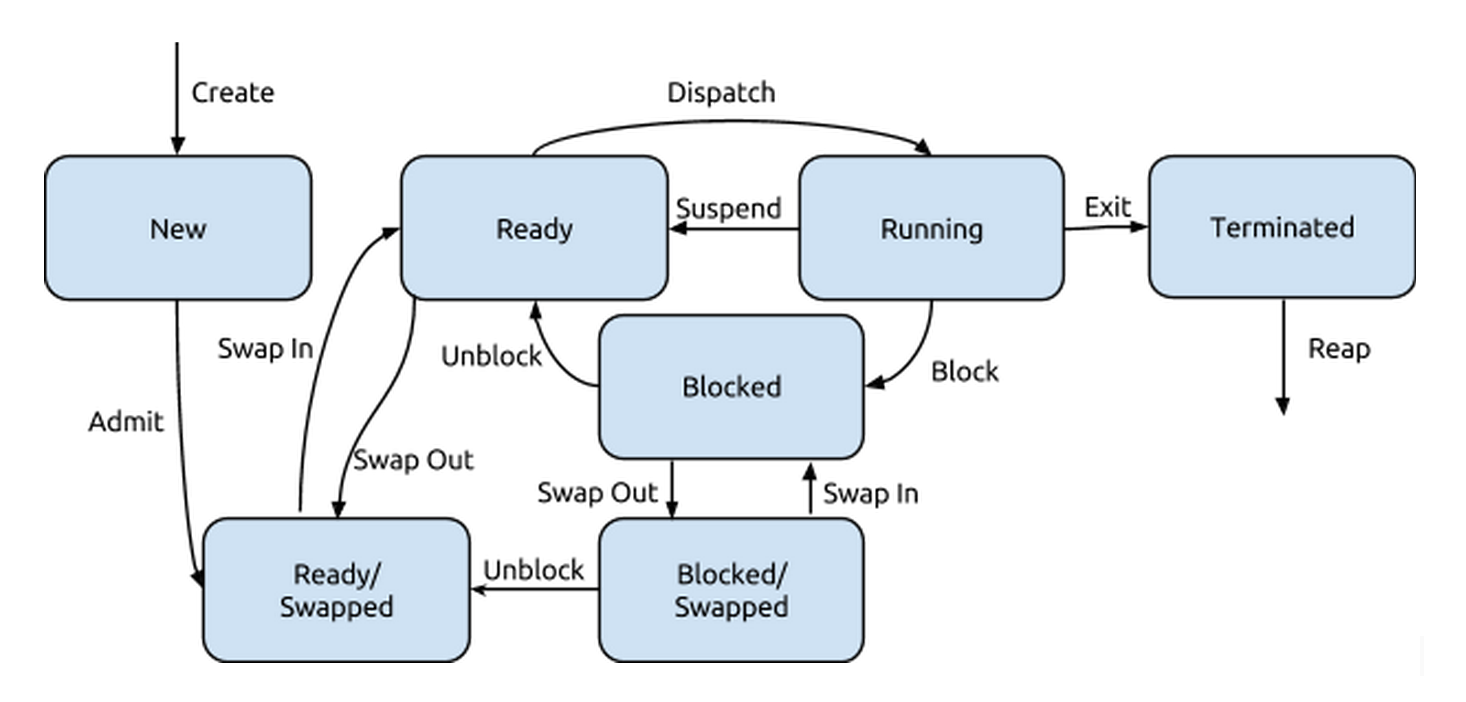
\includegraphics[width=0.9\textwidth]{images/7-state-model.png}
	\end{center}

\end{frame}

\begin{frame}
	\frametitle{Seven State Model}
	A variant of the five state model.

	The ``Admit'' transition is modified: by default the new process does not start in main memory.

	Two new transitions: ``Swap In'' and ``Swap Out''.

	A second ``Unblock'' transition.

	As in the five state model, some additional ``Exit'' transitions.

\end{frame}

\end{document}

